\chapter{Data analysis}\label{sec:data-ana}

The dataset used in this thesis is the Indoor Location \& Navigation from kaggle\cite{kaggle} which was part of a competition of Microsoft Research in 2021\cite{IndoorLocationNavigation}.
The data was recorded in shopping malls by XYZ\(^{10}\) and was provided by Microsoft Research for this competition.
The goal for the competition was, given a site-path file, predict the floor and waypoint locations at a timestamp given in the submission files.
In the following the dataset and data will be analyzed.


\section{Components of the dataset}\label{sec:data}
As noted in the kaggle notebook ``Indoor Navigation: Complete Data Understanding'' \cite{IndoorNavigationUnderstanding} the data consists of 3 parts:
% 
\begin{itemize}
    \item a train folder with train path files, organized by site and floor
    \item a test folder with test path files, organized by site and floor but without waypoint data
    \item a metadata folder with floor metadata, organized by site and floor, which includes floor images, further information and a geojson map
\end{itemize}

The train folder consists of 204 subfolders, which represent each site where the data was recorded.
In each site folder are a minimum of one and a maximum twelve subfolders, which represent the floors of the site, the median is 5 floors.
Overall there are 26,925 files each representing a movement on a specific floor and site.
Per floor, there are between one and 284 files with a median of 14 files.
These files contain the information about the movement of a person on this specific site and floor.
With this amount of data, it could be possible to train a machine learning model.

For this thesis, the submission files as well as the test folder will not be used, because our goal is another type of prediction.


\section{File structure}\label{sec:file-structure}

Each file in each floor folder is a \textbf{.txt} file. 
The first two lines and the last are denoted with ``\#''.
The first contains the start time of the recording, the second site information SiteID as hash, SiteName, FloorId as hash and FloorName.
The last line contains the end time of the recording.
The main part of the data consists of the collected data. 
Each line contains a UNIX timestamp in milliseconds, followed by a data type and the data itself, which are all separated by a tab.
Regard to the GitHub repository\cite{GitHubComp}, the data type in the second column followed by its data can be one of the following:

\setlist[enumerate]{label=(\arabic*)}
\begin{enumerate}
    \item\label{type:acce} TYPE\_ACCELEROMETER with x, y and z acceleration and an accuracy value
    \item\label{type:mag} TYPE\_MAGNETIC\_FIELD with x, y and z magnetic field and an accuracy value
    \item\label{type:gyro} TYPE\_GYROSCOPE with x, y and z gyroscope and an accuracy value
    \item\label{type:rot} TYPE\_ROTATION\_VECTOR with x, y and z rotation vector and an accuracy value
    \item\label{type:mag_u} TYPE\_MAGNETIC\_FIELD\_UNCALIBRATED with x, y and z magnetic field and an accuracy value
    \item\label{type:gyro_u} TYPE\_GYROSCOPE\_UNCALIBRATED with x, y and z gyroscope and an accuracy value
    \item\label{type:acce_u} TYPE\_ACCELEROMETER\_UNCALIBRATED with x, y and z acceleration and an accuracy value
    \item\label{type:wifi} TYPE\_WIFI with \ac{ssid}, \ac{bssid}, \ac{rssi}, frequency, and last seen timestamp of the access point. The SSID and BSSID are hashed.
    \item\label{type:beacon} TYPE\_BEACON with \ac{uuid}, \ac{MajorID}, \ac{MinorID}, \ac{TxPower}, \ac{rssi}, distance to the device measured by the beacon, \ac{mac} address and a timestamp as padding data. The MajorID and MinorID are hashed.
    \item\label{type:way} TYPE\_WAYPOINT with x and y coordinates which are the ground truth location labeled by the surveyor
\end{enumerate}

\lstset{
    basicstyle=\scriptsize\ttfamily,
    breaklines=true,
    escapeinside={(*@}{@*)},
}

\begin{lstlisting}[caption={A snippet of a file from the dataset},label={lst:dataset}]
    #	startTime:1571462193934
    #	SiteID:5d27099303f801723c32364d	SiteName:(*@\begin{CJK*}{UTF8}{gbsn}银泰百货(庆春店)\end{CJK*}@*) FloorId:5d27099303f801723c323650	FloorName:4F
    1571462193944	TYPE_WAYPOINT	57.885998	69.501526
    1571462194071	TYPE_ACCELEROMETER	-0.95254517	0.7944031	8.928757	2
    1571462194071	TYPE_MAGNETIC_FIELD	-25.65918	-4.4784546	-28.201294	3
    1571462194071	TYPE_GYROSCOPE	-0.22373962	-0.07733154	-0.16847229	3
    1571462194071	TYPE_ROTATION_VECTOR	0.04186145	-0.02101801	-0.72491926	3
    1571462194071	TYPE_MAGNETIC_FIELD_UNCALIBRATED	-4.8568726	10.406494	-387.44965	20.802307	14.884949	-359.24835	3
    1571462194071	TYPE_GYROSCOPE_UNCALIBRATED	-0.22218323	-0.068359375	-0.1628418	0.0026245117	9.765625E-4	-7.6293945E-4	3
    1571462194071	TYPE_ACCELEROMETER_UNCALIBRATED	-0.95254517	0.7944031	8.928757	0.0	0.0	0.0	3
    ...
    1571462194883	TYPE_WIFI	b06c4e327882fab58dfa93ea85ca373a54e887b5	9f967858afcbb907af6e5adef766c7e7b936ef07	-63	2462	1571462190744
    1571462194883	TYPE_WIFI	8204870beb9d02995dab3f08aad97af5eab723cc	0413b35df78fc865af15b4721d5aeb33ff57da45	-64	2447	1571462188686
    ...
    1571462194020	TYPE_BEACON	07efd69e3167537492f0ead89fb2779633b04949	b6589fc6ab0dc82cf12099d1c2d40ab994e8410c	76e907e391ad1856762f70538b0fd13111ba68cd	-57	-71	5.002991815535578	1b7e1594febd760b00f1a7984e470867616cee4e	1571462194020
    ...
    #	endTime:1571462195976
\end{lstlisting}

Each site has different amount of floors and also the amount of generated files varies.
Each file contains different amount of waypoints and sensor data.
The first and last data type in each file is a \ref{type:wifi}.
Lines with types from \ref{type:acce} to \ref{type:acce_u} occur every 20 ms.
\(TYPE\_WIFI\)\ref{type:wifi} occurs about every 1800 to 2050 ms.

As seen in \autoref{lst:dataset}, the data are measured separately from each other, so there are no combinations of the data types.
For machine learning it is essential to have all the data for a specific time for a time series.
Especially, \(TYPE\_WAYPOINT\) and \(TYPE\_WIFI\) should be combined to get a location for the \ac{wifi} data point.
For a \(TYPE\_WIFI\) data point a location is not provided.
Furthermore, the \(TYPE\_WAYPOINT\) data points are not evenly distributed as well as there are only 6549 of them in the floor folder with the most files, which is floor 1 of site \begin{CJK*}{UTF8}{gbsn}银泰城(城西店)\end{CJK*} which was hashed as ``5d27075f03f801723c2e360f''.
A movement between these two data points may have occurred.
For a connection between a \(TYPE\_WAYPOINT\) and a \(TYPE\_WIFI\) data point, an interpolation of waypoints between these data points could be useful.
Therefore, this interpolation was made on the data resulting in 
Using linear interpolation of x and y coordinates of the waypoints for the timestamps of \(TYPE\_WIFI\).

This enables a more detailed analysis of the gathered data.

\section{Visualization of one complete floor}\label{sec:visualization}
- visualization of waypoints of one floor without interpolation
%TODO: currently wrong interpolation, fix and compare
\begin{figure}
    \centering
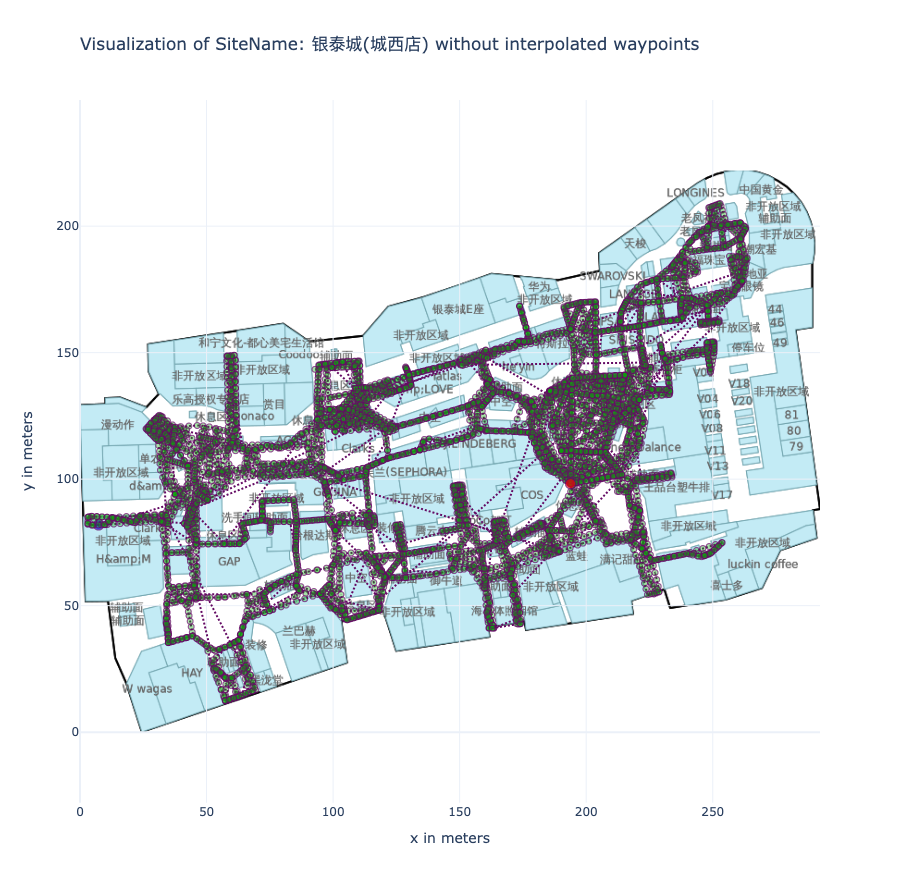
\includegraphics[scale=0.435]{images/whole_floor_visualization_wo_interpolation.png}
\caption[]{Visualization of the waypoints for SiteName: \begin{CJK*}{UTF8}{gbsn}银泰城(城西店)\end{CJK*}}
\end{figure}

- visualization of waypoints of one floor with interpolation
\begin{figure}
        \centering
    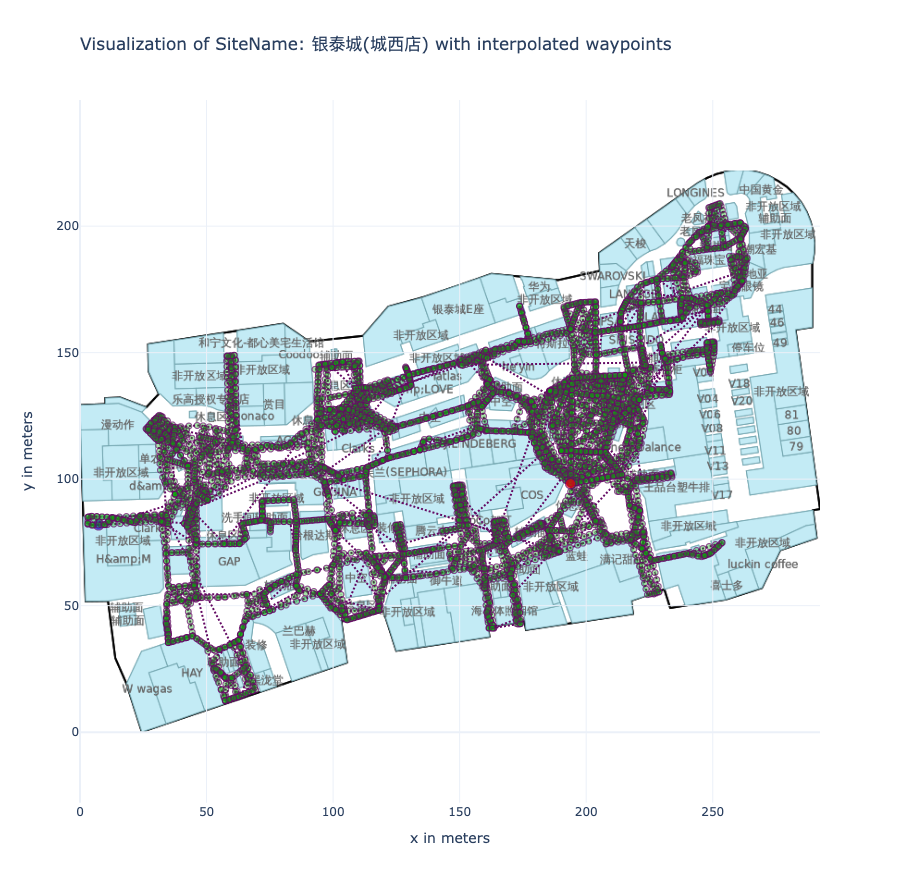
\includegraphics[scale=0.435]{images/whole_floor_visualization_interpolated.png}
    \caption[]{Visualization of the interpolated waypoints for SiteName: \begin{CJK*}{UTF8}{gbsn}银泰城(城西店)\end{CJK*}}
\end{figure}

\section{Peculiarities of the data}\label{sec:special-cases}
Further analysis of the dataset revealed some peculiarities, which are described in the following.

The data is collected by different devices, at different timestamps and days, and one problem for the ML could be, that the waypoint data were measured irregular.

\begin{lstlisting}
1. Timestamp 1: 1572951273212.0, Timestamp 2: 1574853182904.0, Time Difference in ms: 1901909692.0 in min: 31698.494866666668 
2. Timestamp 1: 1571745701735.0, Timestamp 2: 1572937550526.0, Time Difference in ms: 1191848791.0 in min: 19864.146516666668 
3. Timestamp 1: 1571398890607.0, Timestamp 2: 1571745386405.0, Time Difference in ms: 346495798.0 in min: 5774.929966666667 
4. Timestamp 1: 1571222697051.0, Timestamp 2: 1571393792128.0, Time Difference in ms: 171095077.0 in min: 2851.5846166666665 
5. Timestamp 1: 1572947759794.0, Timestamp 2: 1572950695861.0, Time Difference in ms: 2936067.0 in min: 48.93445 
6. Timestamp 1: 1572942316535.0, Timestamp 2: 1572944901430.0, Time Difference in ms: 2584895.0 in min: 43.081583333333334 
7. Timestamp 1: 1572946047608.0, Timestamp 2: 1572947705343.0, Time Difference in ms: 1657735.0 in min: 27.628916666666665 
8. Timestamp 1: 1572938081167.0, Timestamp 2: 1572938843518.0, Time Difference in ms: 762351.0 in min: 12.70585 
9. Timestamp 1: 1571397963778.0, Timestamp 2: 1571398570240.0, Time Difference in ms: 606462.0 in min: 10.1077 
10. Timestamp 1: 1572937620091.0, Timestamp 2: 1572938025654.0, Time Difference in ms: 405563.0 in min: 6.759383333333333 
\end{lstlisting}

